\documentclass{beamer}
%\setbeamertemplate{items}[ball] 
\DeclareMathOperator*{\argmax}{arg\,max}
\usecolortheme{whale}
\useinnertheme[shadow]{rounded}
\usenavigationsymbolstemplate{}
\usepackage[subsection=false,headline=empty,footline=outlineauthortitle]{beamerouterthememiniframesbottom}
%\usepackage{beamerthemesplit}
\usepackage{tikz}
\usepackage{pgfplots}
\usetikzlibrary{arrows,automata,positioning,shapes,shapes.geometric,fit,tikzmark}
\usefonttheme[onlymath]{serif}

\usepackage{enumitem}

\usepackage{textcomp}
% Set up citation style
\usepackage{natbib}
\usepackage{bibentry}
\bibpunct{(}{)}{;}{a}{,}{,}
\newcommand{\newcite}[1]{\citet{#1}}
\renewcommand{\cite}[1]{\citep{#1}}

%\setbeamercovered{transparent}

% Specify that no bibliography should be printed
\bibliographystyle{plainnat}


\setbeamertemplate{footline}[frame number]{}

%gets rid of bottom navigation symbols
\setbeamertemplate{navigation symbols}{}

%gets rid of footer
%will override 'frame number' instruction above
%comment out to revert to previous/default definitions
\setbeamertemplate{footline}{}

\usepackage{pgfpages}
\usepackage{graphicx}
\usepackage{enumitem}
\setlist[itemize,1]{label={\fontfamily{cmr}\fontencoding{T1}\selectfont\textbullet}}


%\setbeamertemplate{note page}[plain]
%\setbeameroption{show notes on second screen=right}
%\usepackage{minted}
\title{Neural Network Concepts}
%\author{Lane Schwartz}

%\institute[shortinst]{University of Illinois at Urbana-Champaign}

\author{Biological and Artificial Neurons}

\date{}

\begin{document}

\frame{
\titlepage

}

\frame{\frametitle{Biology}

  \begin{itemize}
    \item Brain is complex, made of thousands or millions of interconnected cells
    \item Neurons are slow compared to computers (milliseconds vs nanoseconds)
    \item Nevertheless, brains can do things that computers can't
    \item Processing in the brain appears to be massively parallel
    \item Brains have redundancies
  \end{itemize}

}

\frame{\frametitle{Anatomy of a biological neuron}
  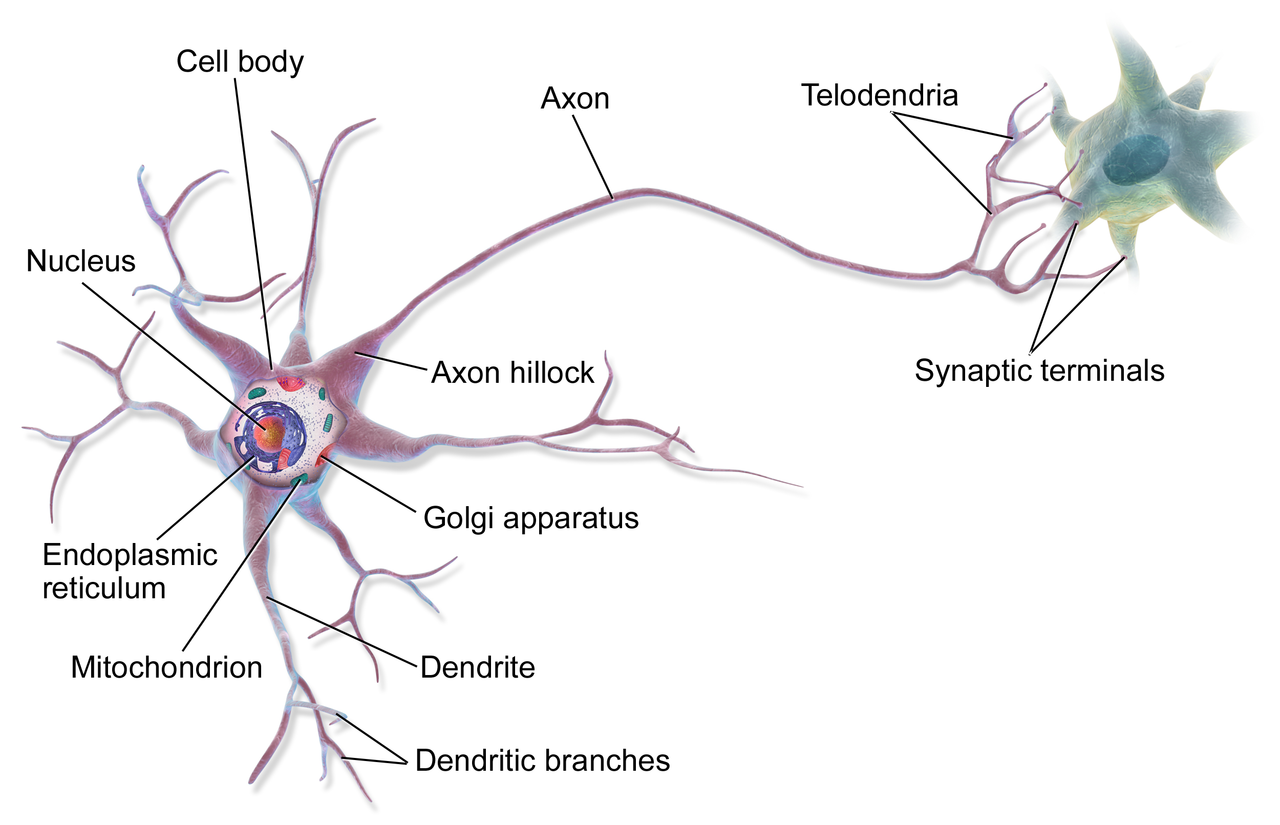
\includegraphics[width=\textwidth]{images/Blausen_0657_MultipolarNeuron}

  \tiny{\url{https://commons.wikimedia.org/wiki/File:Blausen_0657_MultipolarNeuron.png}}
}

\frame{\frametitle{Networks of biological neurons}

  \begin{center}
    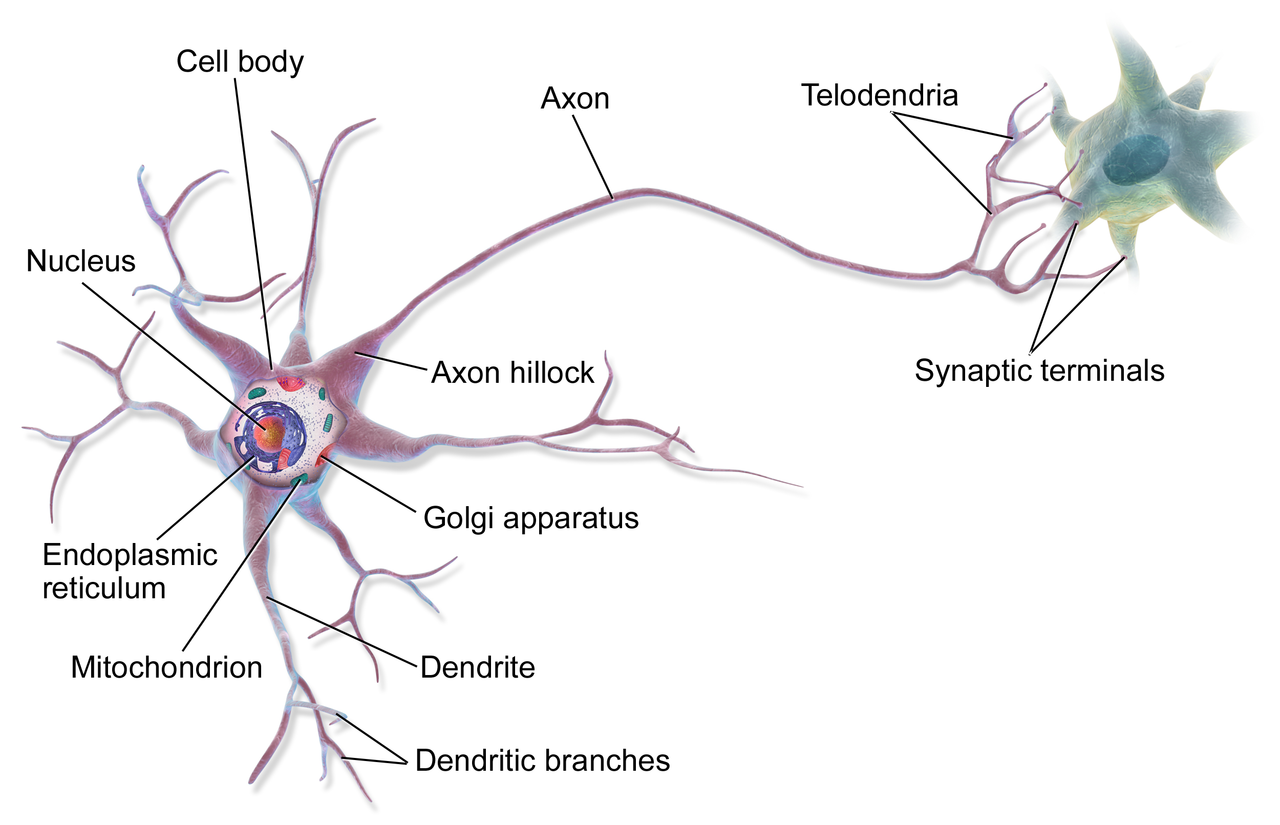
\includegraphics[width=0.5\textwidth]{images/Blausen_0657_MultipolarNeuron}
  \end{center}
  
  \begin{itemize}
    \item Outgoing signal transmitted along \textbf{axon}
    \item \textbf{Synapse} is a connection point between neurons
    \item Incoming signals received at \textbf{dendrite}
  \end{itemize}

}

\frame{\frametitle{Networks of biological neurons}

  \begin{center}
    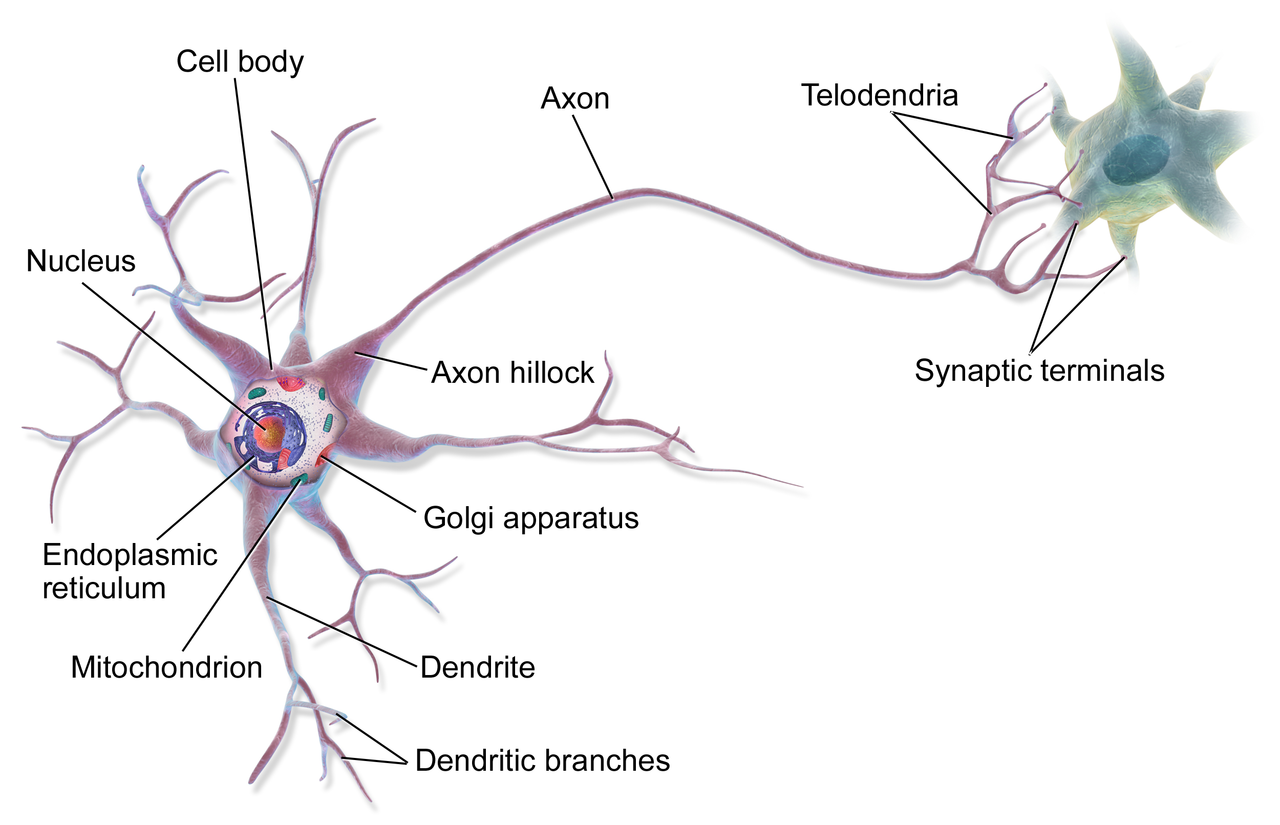
\includegraphics[width=0.5\textwidth]{images/Blausen_0657_MultipolarNeuron}
  \end{center}
  
  \begin{itemize}
    \item Electro-chemical signals propagate between neurons
    \item Frequency modulation (FM)
    \item Synaptic connections vary in strength (weight)
  \end{itemize}

}

\frame{\frametitle{Anatomy of an artificial neuron}

  \begin{center}
  \begin{tikzpicture}
    [neuron/.style={circle,draw=black,fill=white,inner sep=0pt,minimum size=10mm,outer sep=0.5pt},
    >=stealth',
    scale=0.7,transform shape]
    
    \node (i01)                              {$i_1$};
    \node (i02)      [below=5mm of i01]      {$i_2$};
    \node (i_hidden) [below=5mm of i02]      {\vdots};
    \node (i03)      [below=5mm of i_hidden] {\ };
    \node (i0n)      [below=5mm of i03]      {$i_n$};
    
    \node[neuron] (n01) [right=20mm of i_hidden] {$f$};
    
    \node (out)      [right=20mm of n01] {$f(\sum_{i=1}^n w_i x_i)$};
    
    \draw [->] (i01) -- (n01) node [midway,above=0.5mm] {$w_1$};
    \draw [->] (i02) -- (n01) node [midway,below=0.5mm] {$w_2$};
    \draw [->] (i0n) -- (n01) node [midway,below=0.5mm] {$w_n$};
    \draw [->]  (n01) -- (out);
    
  \end{tikzpicture}
  \end{center}

  Artificial neurons are extremely simplified models

  \begin{itemize}
    \item Incoming edges roughly correspond to denrites
    \item Outgoing edge roughly corresponds to axon
    \item Incoming edge weights roughly correspond to strength of synaptic connection
  \end{itemize}

}


\frame{\frametitle{Networks of artificial neurons}

  \begin{center}
  \begin{tikzpicture}
    [neuron/.style={circle,draw=black,fill=white,inner sep=0pt,minimum size=10mm,outer sep=0.5pt},
    >=stealth',
    scale=0.7,transform shape]
    
    \node          (i01)                              {$i_1$};
    
    \node [neuron] (n01)      [right=20mm of i01]     {$f_1$};
    \node [neuron] (n02)      [below=10mm of n01]     {$f_2$};

    \node          (i02)      [left=20mm of n02]      {$i_2$};
    

    \node [neuron] (n03)      [right=20mm of n01]     {$f_3$};
    \node          (inv)      [below=5mm of  n03]     {\ };
    \node [neuron] (n04)      [right=20mm of n02]     {$f_4$};

    \node [neuron] (n05)      [right=20mm of inv]     {$f_5$};
    
    \node (out)      [right=20mm of n05] {$o$};
    
    \draw [->] (i01) -- (n01);
    \draw [->] (i02) -- (n01);
    
    \draw [->] (i01) -- (n02);
    \draw [->] (i02) -- (n02);
    
    \draw [->] (n01) -- (n03);
    \draw [->] (n02) -- (n03);
    
    \draw [->] (n01) -- (n04);
    \draw [->] (n02) -- (n04);
    
    \draw [->] (n03) -- (n05);
    \draw [->] (n04) -- (n05);
    
    \draw [->] (n05) -- (out);
    
  \end{tikzpicture}
  \end{center}

  Artificial neural networks

  \begin{itemize}
    \item We must specify the function $f$
    \item We must specify the network topology \\ (how many nodes, how they are connected)
    \item We must specify a learning algorithm
    \item We will learn the weights
  \end{itemize}

}


\frame{\frametitle{Networks of artificial neurons}

  \begin{center}
  \begin{tikzpicture}
    [neuron/.style={circle,draw=black,fill=white,inner sep=0pt,minimum size=10mm,outer sep=0.5pt},
    >=stealth',
    scale=0.7,transform shape]
    
    \node          (i01)                              {$i_1$};
    
    \node [neuron] (n01)      [right=20mm of i01]     {$f_1$};
    \node [neuron] (n02)      [below=10mm of n01]     {$f_2$};

    \node          (i02)      [left=20mm of n02]      {$i_2$};
    

    \node [neuron] (n03)      [right=20mm of n01]     {$f_3$};
    \node          (inv)      [below=5mm of  n03]     {\ };
    \node [neuron] (n04)      [right=20mm of n02]     {$f_4$};

    \node [neuron] (n05)      [right=20mm of inv]     {$f_5$};
    
    \node (out)      [right=20mm of n05] {$o$};
    
    \draw [->] (i01) -- (n01);
    \draw [->] (i02) -- (n01);
    
    \draw [->] (i01) -- (n02);
    \draw [->] (i02) -- (n02);
    
    \draw [->] (n01) -- (n03);
    \draw [->] (n02) -- (n03);
    
    \draw [->] (n01) -- (n04);
    \draw [->] (n02) -- (n04);
    
    \draw [->] (n03) -- (n05);
    \draw [->] (n04) -- (n05);
    
    \draw [->] (n05) -- (out);
    
  \end{tikzpicture}
  \end{center}

  Artificial neural networks

  \begin{itemize}
    \item Each artificial neuron (with its associated weights) \\ specifies a function
	\item The entire neural network (with its associated weights) specifies a more complex function
  \end{itemize}

}


\frame{\frametitle{The Big Picture}

  A neural network is a \textbf{function approximator}

  \begin{itemize}
    \item We begin with training data (input-output pairs)
  	\item We design a network topology
	\item We select a learning algorithm
	\item We learn the network weights \\ (using training data \& learning algorithm)
  \end{itemize}  

  \ \\

  \ \\
  
  The result is a trained neural network capable of approximating the function which produced the input-output pairs.

}

\begin{frame}

\note{
This presentation was created and narrated by Lane Schwartz. \\ \ \\
You are free to reproduce and adapt this work under the terms of the Creative Commons Attribution-ShareAlike 4.0 International License.
}

\begin{center}

\includegraphics[scale=0.3]{images/CreativeCommons} \ \ \ \ \ 

\includegraphics[scale=0.3]{images/CreativeCommonsAttribution} \ \ \ \ \ 

\includegraphics[scale=0.3]{images/CreativeCommonsSharealike}
\end{center}

\ \\

%\setbeamertemplate{itemize items}[$+$]
\begin{itemize}
\item[\textbullet] This presentation was created and narrated by Lane Schwartz. \\ \ \\
\item[\textbullet] You are free to reproduce and adapt this work under the terms of the Creative Commons Attribution-ShareAlike 4.0 International License.
\end{itemize}

\end{frame}


%\begin{frame}
\frametitle{Linear unit}

\begin{equation*}
y = b + \sum_i x_i w_i
\end{equation*}


\begin{tikzpicture}
\begin{axis}[ylabel=output,xlabel=weighted input,scale=0.3,grid=major,ytick={0},xtick={0},xmin=-5,xmax=5,ymin=-5,ymax=5]
  \addplot[blue, ultra thick][domain=-10:10] (x,x);
\end{axis}
\end{tikzpicture}

\end{frame}


%\frame {

\begin{center}
$f(x_1,x_2) = \sin(x_1) + x_1*x_2$ \ \ \ \ \ \ \ \ \ \ 
$\bar{x_i} = \frac{\partial f_j}{\partial x_i}$
\pause

\begin{tikzpicture}[>=latex, scale=0.75, transform shape]
\tikzstyle{every node}=[font=\large]
\tikzstyle{every path}=[line width=1pt]

\node[state,rectangle] (fxx) {$f(x_1,x_2)$};
\node[state] (plus) [below=1.5cm of fxx] {$f_5$};
\node[state] (sin) [below left=1.5cm and 0.5cm of plus] {$f_4$};
\node[state] (mul) [below right=1.5cm and 0.5cm of plus] {$f_3$};
\node[state] (x1) [below left=1.5cm and 0.5 cm of sin] {$f_1$};
\node[state] (x2) [below right=1.5cm and 0.5 cm of mul] {$f_2$};

\onslide<+>{
\path[-]
(plus) edge node {} (fxx)
(sin) edge node {} (plus)
(mul) edge node {} (plus)
(x1) edge node {} (sin)
(x1) edge node {} (mul)
(x2) edge node {} (mul);
}

\onslide<+>{
\path[->,blue]
(plus) edge node {} (fxx)
(sin) edge node {} (plus)
(mul) edge node {} (plus)
(x1) edge node {} (sin)
(x1) edge node {} (mul)
(x2) edge node {} (mul);
}

\onslide<.->{
\node[state, draw=none,fill=none,blue] (w1) [left=0.1cm of x1] {$y_1 = f_1(x_1) = x_1$};
\node[state, draw=none,fill=none,blue] (w2) [right=0.1cm of x2] {$y_2 = f_2(x_2) = x_2$};
\node[state, draw=none,fill=none,blue] (w3) [right=0.1cm of mul] {$y_3 = f_3(y_1, y_2) = y_1 \cdot y_2$};
\node[state, draw=none,fill=none,blue] (w4) [left=0.1cm of sin] {$y_4 = f_4(y_1) = \sin(y_1)$};
\node[state, draw=none,fill=none,blue] (w5) [left=0.1cm of plus] {$y_5 = f_5(y_3, y_4) = y_3 + y_4$};
\node[state, draw=none,fill=none,blue] (w6) [right=0.1cm of fxx] {$y_6 = f_6(y_5) = y_5$};
}

\onslide<+>{
\path[<-,red]
(plus) edge node [right] {$\bar{f_6} = \bar{y}_5 = \frac{\partial f_6}{\partial y_5} = 1$} (fxx)
(sin) edge node [left, pos=.6] {$\bar{y}_4 = \frac{\partial f_6}{\partial y_4} = \frac{\partial f_6}{\partial y_5} \frac{\partial y_5}{\partial y_4} = \bar{y}_5 \frac{\partial f_5}{\partial y_4} = \bar{y}_5 \cdot 1 = \bar{y}_5$} (plus)
(mul) edge node [right, pos=.6] {$\bar{y}_3 = \frac{\partial f_6}{\partial y_3} = \frac{\partial f_6}{\partial y_5} \frac{\partial y_5}{\partial y_3} = \bar{y}_5 \frac{\partial f_5}{\partial y_3} = \bar{y}_5 \cdot 1 = \bar{y}_5$} (plus)
(x1) edge node [left,pos=.6] { $\frac{\partial f_6}{\partial y_1} = \bar{y}_4 \frac{\partial y_4}{\partial y_1} = \bar{y}_4\cdot\cos(y_1)$ } (sin)
(x1) edge node [right, pos=.3] {$\bar{y}_{1^b}= \bar{y}_3\cdot y_2$} (mul)
(x2) edge node [right, pos=.6] {$\bar{y}_2 = \bar{y}_3 \frac{\partial y_3}{\partial y_2} = \bar{y}_3\cdot y_1$} (mul);

}

\end{tikzpicture}
\end{center}
}




\frame {

\begin{center}
$f(x_1,x_2) = \sin(x_1) + x_1*x_2$

\ \\

\pause

\begin{tikzpicture}[>=latex, scale=0.75, transform shape]
\tikzstyle{every node}=[font=\large]
\tikzstyle{every path}=[line width=1pt]

\node[state,rectangle] (fxx) {$f(x_1,x_2)$};
\node[state] (plus) [below=1.5cm of fxx] {$+$};
\node[state] (sin) [below left=1.5cm and 0.5cm of plus] {$\sin$};
\node[state] (mul) [below right=1.5cm and 0.5cm of plus] {$*$};
\node[state,rectangle] (x1) [below left=1.5cm and 0.5 cm of sin] {$x_1$};
\node[state,rectangle] (x2) [below right=1.5cm and 0.5 cm of mul] {$x_2$};

\onslide<+>{
\path[-]
(plus) edge node {} (fxx)
(sin) edge node {} (plus)
(mul) edge node {} (plus)
(x1) edge node {} (sin)
(x1) edge node {} (mul)
(x2) edge node {} (mul);
}

\onslide<+>{
\path[->,blue]
(plus) edge node {} (fxx)
(sin) edge node {} (plus)
(mul) edge node {} (plus)
(x1) edge node {} (sin)
(x1) edge node {} (mul)
(x2) edge node {} (mul);
}

\onslide<.->{
\node[state, draw=none,fill=none,blue] (w1) [left=0.1cm of x1] {$y_1 = x_1$};
\node[state, draw=none,fill=none,blue] (w2) [right=0.1cm of x2] {$y_2 = x_2$};
\node[state, draw=none,fill=none,blue] (w3) [right=0.1cm of mul] {$y_3 = y_1 \cdot y_2$};
\node[state, draw=none,fill=none,blue] (w4) [left=0.1cm of sin] {$y_4 = \sin(y_1)$};
\node[state, draw=none,fill=none,blue] (w4) [left=0.1cm of plus] {$y_5 = y_3 + y_4$};
}

\onslide<+>{
\path[<-,red]
(plus) edge node [right] {$\bar{f} = \bar{y}_5 = \frac{\partial f}{\partial y_5} = 1$} (fxx)
(sin) edge node [left, pos=.6] {$\bar{y}_4 = \bar{y}_5 \frac{\partial y_5}{\partial y_4}$} (plus)
(mul) edge node [right, pos=.6] {$\bar{y}_3 = \bar{y}_5 \frac{\partial y_5}{\partial y_3}$} (plus)
(x1) edge node [left,pos=.6] { $\bar{y}_1^a = \bar{y}_4 \frac{\partial y_4}{\partial y_1} = \bar{y}_4\cdot\cos(y_1)$ } (sin)
(x1) edge node [right, pos=.3] {$\bar{y}_1^b= \bar{y}_3\cdot y_2$} (mul)
(x2) edge node [right, pos=.6] {$\bar{y}_2 = \bar{y}_3 \frac{\partial y_3}{\partial y_2} = \bar{y}_3\cdot y_1$} (mul);

}


\end{tikzpicture}
\end{center}
}



\end{document}
